%
% 01_satz.tex -- Einfuhrung in den Satz von Jordan
%
% (c) 2026 Dominik Castelberg, Ostschweizer Fachhochschule
%
% !TEX root = ../../buch.tex
% !TEX encoding = UTF-8
%
\section{Der Satz von Jordan \label{jordan:section:01_satz}}
\kopfrechts{Der Satz von Jordan}

Die meisten Sätze der höheren Mathematik setzen ein tiefes Verständnis der zugrunde liegenden mathematischen Strukturen voraus, damit über ihre Korrektheit argumentiert werden kann. 
Andere Sätze erscheinen jedoch derart trivial, dass ihre Korrektheit auf den ersten Blick offensichtlich ist und man zum Fehlschluss kommen könnte, dass ein Beweis überflüssig ist. 
Der Satz von Jordan ist einer dieser vermeintlich trivialen Sätze.

\begin{satz}[Satz von Jordan\label{jordan:satz:jordan}]
    Sei $\gamma$ eine einfache geschlossene Kurve in der Ebene $\mathbb{R}^2$. 
    Dann teilt $\gamma$ die Ebene in genau zwei zusammenhängende Gebiete: ein inneres Gebiet, das von $\gamma$ eingeschlossen wird, und ein äusseres Gebiet, das unendlich ausgedehnt ist. 
    Die Kurve $\gamma$ selbst bildet der gemeinsame Rand dieser beiden Gebiete.
\end{satz}

Der Begriff der einfachen geschlossenen Kurve schränkt den Gültigkeitsbereich des Satzes von Jordan auf Kurven, welche eine Schleife bilden und sich dabei nicht selbst schneiden, ein.

\begin{definition}[einfache geschlossene Kurve\label{jordan:definition:einfache_geschlossene_kurve}]
    Eine einfache geschlossene Kurve $\gamma$ in der Ebene $\mathbb{R}^2$ ist eine stetige Abbildung $\gamma: [0,1] \to \mathbb{R}^2$, die folgende Eigenschaften erfüllt:
    \begin{enumerate}
        \item $\gamma(0) = \gamma(1)$.
        \item $\gamma(t_1) \neq \gamma(t_2)$ für alle $t_1, t_2 \in [0,1)$ mit $t_1 \neq t_2$.
    \end{enumerate}
\end{definition}

Später werden wir Kurven, für welche der Satz von Jordan gilt, auch als Jordan-Kurven bezeichnen.

\begin{figure}
    \centering
    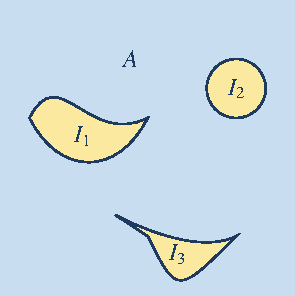
\includegraphics{papers/jordan/images/jordan_kurve.pdf}
    \caption{Beispiele für einfache geschlossene Kurven, welche die Ebene in innere Gebiete $I_1, I_2, I_3$ und ein äusseres Gebiet $A$ unterteilen.}
\end{figure}

Das Satz von Jordan gehört zu den fundamentalen Resultaten der Topologie und hat weitreichende Anwendungen in verschiedenen Bereichen der Mathematik, der Physik und der Informatik. 
Seit seiner Formulierung im Jahr 1887 durch Camille Jordan versuchten Mathematiker, den Satz zu beweisen, wobei die ersten Versuche jeweils nach kurzer Zeit wieder verworfen wurden. 
Die Beweise waren oft unvollständig oder fehlerhaft, und es dauerte mehrere Jahrzehnte, bis der erste, allgemein als vollständig und rigoros anerkannte Beweis durch Oswald Veblen im Jahr 1905 veröffentlicht wurde.

Was macht diesen Satz so schwierig zu beweisen?
Die Schwierigkeit liegt primär in der allgemeinen Formulierung des Satzes. Während es geradezu trivial ist, den Satz für spezielle Kurvenformen wie Kreise oder Ellipsen zu beweisen, wird die Komplexität des Beweises grösser, wenn man die Bedingung der Einfachheit und Geschlossenheit auf beliebige Kurven anwendet.
Stetigkeit wirkt nur als eine schwache Einschränkung auf die Kurve und erlaubt wilde Formen wie Fraktale, raumfüllende Kurven im Inneren oder Ränder mit positivem Lebesgue-Mass.
Die Implikationen der Eigenschaften dieser Beispiele sind über menschliche Intuition nur schwer zu erfassen.
Aber wie wir später sehen werden, sind solche Kurven enorm aufwändig zu analysieren, was die Beweisführung für den Satz von Jordan deutlich erschwert. 